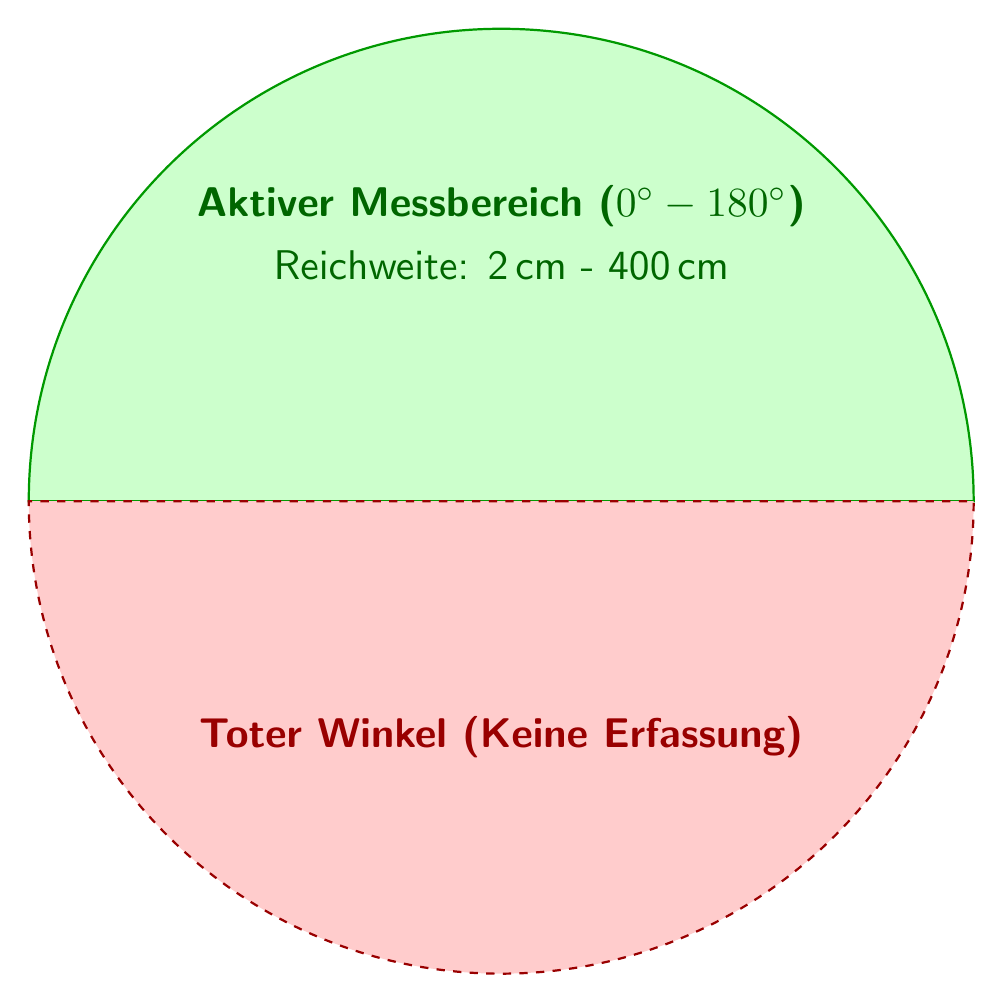
\begin{tikzpicture}[font=\sffamily, scale=1.5, transform shape]
	% Sensor in der Mitte
	\filldraw[fill=gray!50, draw=black, thick] (-0.5,-0.5) rectangle (0.5,0.5);
	\node at (0,0) {\textbf{Radar}};
	
	% Aktiver Bereich (oben)
	\filldraw[fill=green!20, draw=green!60!black, thick] (0.5,0) -- (4,0) arc (0:180:4) -- (-0.5,0) -- cycle;
	\node[text=green!40!black] at (0, 2.5) {\textbf{Aktiver Messbereich ($0^\circ - 180^\circ$)}};
	\node[text=green!40!black] at (0, 2) {Reichweite: 2\,cm - 400\,cm};
	
	% Toter Winkel (unten)
	\filldraw[fill=red!20, draw=red!60!black, thick, dashed] (0.5,0) -- (4,0) arc (360:180:4) -- (-0.5,0) -- cycle;
	\node[text=red!60!black] at (0, -2) {\textbf{Toter Winkel (Keine Erfassung)}};
\end{tikzpicture}